\chapter{Techno-Economic Analysis}
\label{sec: techo-analysis}
    % \begin{landscape}
        \section{Planning}
        \begin{figure} [H]
        % \vspace*{1cm}
        % \hspace*{-3cm}
        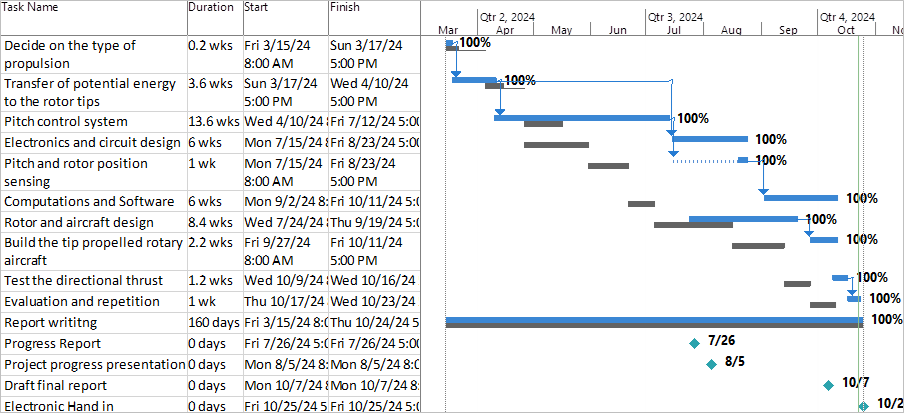
\includegraphics[width = \linewidth]{figs/Gantt Charts/Final_Rerport_Gantt.png}
        \caption{Gantt Chart for project}
        \label{fig: gantt_chart}
        \end{figure}
        The Gantt chart shows the proposed time to complete the tasks with the gray line and the actual start and finish time in blue. It shows that in the beginning the tasks were being completed ahead of the scheduled time until the task `Pitch control system'. This task was originally thought to be looking into the different control methods. While researching lead/lag compensators and state space, a mathematical model was created. This model became more complex in the attempt to make it as accurate as possible, which resulted in it taking longer time then expected. The rest of the activities have been shifted due to this. The build started later than what was originally planned, this was due to issues in obtaining the motors, which delayed part of the build. While the tasks did take longer than expected and were not as planned, all the tasks were completed before the final due date.
\pagebreak
        \section{Budget}

% \begin{landscape}

\begin{table}[H]
    \scriptsize
    \caption{Proposed budget for project}
    \label{tab: proposed_Budget}
    \hspace*{-8.25mm}
    \begin{tabular}{|p{3.5cm}|rr|p{8mm}|p{8mm}|p{7mm}|rrr|p{8.5mm}|}
    \hline
    \multicolumn{1}{|c|}{\multirow{2}{*}{\textbf{Activity}}}                                 & \multicolumn{2}{c|}{\multirow{2}{*}{\textbf{\begin{tabular}[c]{@{}c@{}}Engineering \\ Time\end{tabular}}}} & \multicolumn{1}{c|}{\multirow{2}{*}{\textbf{\begin{tabular}[p{8mm}]{@{}c@{}}Running \\ Costs\end{tabular}}}} & \multicolumn{1}{c|}{\multirow{2}{*}{\textbf{\begin{tabular}[c]{@{}c@{}}Facility \\ Use\end{tabular}}}} & \multicolumn{1}{c|}{\multirow{2}{*}{\textbf{\begin{tabular}[c]{@{}c@{}}Capital \\ Costs\end{tabular}}}} & \multicolumn{3}{c|}{\textbf{MMW}}                                                                              & \multicolumn{1}{l|}{\multirow{2}{*}{\textbf{Total}}} \\ \cline{7-9}
    \multicolumn{1}{|c|}{}                                                                   & \multicolumn{2}{c|}{}                                                                                      & \multicolumn{1}{c|}{}                                                                                   & \multicolumn{1}{c|}{}                                                                                  & \multicolumn{1}{c|}{}                                                                                   & \multicolumn{2}{p{8mm}|}{\textbf{Labour}}                                  & \multicolumn{1}{l|}{\textbf{Material}} & \multicolumn{1}{l|}{}                                \\ \hline
                                                                                             & \multicolumn{1}{l|}{\textbf{hr}}                      & \multicolumn{1}{l|}{\textbf{R}}                    & \multicolumn{1}{l|}{\textbf{R}}                                                                         & \multicolumn{1}{l|}{\textbf{R}}                                                                        & \multicolumn{1}{l|}{\textbf{R}}                                                                         & \multicolumn{1}{l|}{\textbf{hr}} & \multicolumn{1}{l|}{\textbf{R}}    & \multicolumn{1}{l|}{\textbf{R}}        & \multicolumn{1}{l|}{\textbf{R}}                      \\ \hline
    \begin{tabular}[c]{@{}l@{}}Decide on the type\\ of propulsion\end{tabular}               & \multicolumn{1}{r|}{25}                               & 10000                                              & 150                                                                                                     & -                                                                                                      & -                                                                                                       & \multicolumn{1}{r|}{-}           & \multicolumn{1}{r|}{-}             & -                                      & \textbf{10150}                                       \\ \hline
    \begin{tabular}[c]{@{}l@{}}Transfer of potential\\ energy to the rotor\end{tabular}      & \multicolumn{1}{r|}{25}                               & 10000                                              & 300                                                                                                     & -                                                                                                      & -                                                                                                       & \multicolumn{1}{r|}{-}           & \multicolumn{1}{r|}{-}             & -                                      & \textbf{10300}                                       \\ \hline
    Pitch control system                                                                     & \multicolumn{1}{r|}{60}                               & 24000                                              & -                                                                                                       & -                                                                                                      & -                                                                                                       & \multicolumn{1}{r|}{-}           & \multicolumn{1}{r|}{-}             & -                                      & \textbf{24000}                                       \\ \hline
    Electronics and circuit diagram                                                                                  & \multicolumn{1}{r|}{25}                               & 10000                                              & -                                                                                                       & -                                                                                                      & -                                                                                                       & \multicolumn{1}{r|}{-}           & \multicolumn{1}{r|}{-}             & -                                      & \textbf{10000}                                       \\ \hline
    \begin{tabular}[c]{@{}l@{}}Pitch and rotor position \\ sensing\end{tabular}              & \multicolumn{1}{r|}{25}                               & 10000                                              & 100                                                                                                     & 150                                                                                                    & -                                                                                                       & \multicolumn{1}{r|}{-}           & \multicolumn{1}{r|}{-}             & -                                      & \textbf{10250}                                       \\ \hline
    Computations and software                                                                               & \multicolumn{1}{r|}{25}                               & 10000                                              & 250                                                                                                     & -                                                                                                      & -                                                                                                       & \multicolumn{1}{r|}{-}           & \multicolumn{1}{r|}{-}             & -                                      & \textbf{10250}                                       \\ \hline
    Rotor and aircraft design                                                                & \multicolumn{1}{r|}{100}                              & 40000                                              & -                                                                                                       & 200                                                                                                    & -                                                                                                       & \multicolumn{1}{r|}{5}           & \multicolumn{1}{r|}{1500}          & 250                                    & \textbf{41950}                                       \\ \hline
    \begin{tabular}[c]{@{}l@{}}Build the tip propelled \\ rotary aircraft\end{tabular}       & \multicolumn{1}{r|}{70}                               & 28000                                              & -                                                                                                       & -                                                                                                      & -                                                                                                       & \multicolumn{1}{r|}{20}          & \multicolumn{1}{r|}{6000}          & 1500                                   & \textbf{35500}                                       \\ \hline
    Test the directional thrust                                                              & \multicolumn{1}{r|}{15}                               & 6000                                               & 600                                                                                                     & 250                                                                                                    & -                                                                                                       & \multicolumn{1}{r|}{-}           & \multicolumn{1}{r|}{-}             & -                                      & \textbf{6850}                                        \\ \hline
    Evaluation and repetition                                                                & \multicolumn{1}{r|}{15}                               & 6000                                               & -                                                                                                       & 250                                                                                                    & -                                                                                                       & \multicolumn{1}{r|}{-}           & \multicolumn{1}{r|}{-}             & -                                      & \textbf{6250}                                        \\ \hline
    Report writing                                                                           & \multicolumn{1}{r|}{100}                              & 40000                                              & -                                                                                                       & -                                                                                                      & -                                                                                                       & \multicolumn{1}{r|}{-}           & \multicolumn{1}{r|}{-}             & -                                      & \textbf{40000}                                       \\ \hline
    \multicolumn{1}{|r|}{\textbf{Total}}                                                     & \multicolumn{1}{r|}{\textbf{485}}                     & \textbf{194000}                                    & \textbf{1400}                                                                                           & \textbf{850}                                                                                           & \textbf{0}                                                                                              & \multicolumn{1}{r|}{\textbf{25}} & \multicolumn{1}{r|}{\textbf{7500}} & \textbf{1750}                          & \textbf{205500}                                      \\ \hline
    \end{tabular}
    \end{table}
    \normalsize
    \begin{table}[H]
        \scriptsize
        \caption{Actual budget for project}
        \label{tab: actual_Budget}
        \hspace*{-8.25mm}
        \begin{tabular}{|p{3.5cm}|rr|p{8mm}|p{8mm}|p{7mm}|rrr|p{8.5mm}|}
        \hline
        \multicolumn{1}{|c|}{\multirow{2}{*}{\textbf{Activity}}}                                 & \multicolumn{2}{c|}{\multirow{2}{*}{\textbf{\begin{tabular}[c]{@{}c@{}}Engineering \\ Time\end{tabular}}}} & \multicolumn{1}{c|}{\multirow{2}{*}{\textbf{\begin{tabular}[p{8mm}]{@{}c@{}}Running \\ Costs\end{tabular}}}} & \multicolumn{1}{c|}{\multirow{2}{*}{\textbf{\begin{tabular}[c]{@{}c@{}}Facility \\ Use\end{tabular}}}} & \multicolumn{1}{c|}{\multirow{2}{*}{\textbf{\begin{tabular}[c]{@{}c@{}}Capital \\ Costs\end{tabular}}}} & \multicolumn{3}{c|}{\textbf{MMW}}                                                                              & \multicolumn{1}{l|}{\multirow{2}{*}{\textbf{Total}}} \\ \cline{7-9}
        \multicolumn{1}{|c|}{}                                                                   & \multicolumn{2}{c|}{}                                                                                      & \multicolumn{1}{c|}{}                                                                                   & \multicolumn{1}{c|}{}                                                                                  & \multicolumn{1}{c|}{}                                                                                   & \multicolumn{2}{p{8mm}|}{\textbf{Labour}}                                  & \multicolumn{1}{l|}{\textbf{Material}} & \multicolumn{1}{l|}{}                                \\ \hline
                                                                                                 & \multicolumn{1}{l|}{\textbf{hr}}                     & \multicolumn{1}{l|}{\textbf{R}}                    & \multicolumn{1}{l|}{\textbf{R}}                                                                         & \multicolumn{1}{l|}{\textbf{R}}                                                                        & \multicolumn{1}{l|}{\textbf{R}}                                                                         & \multicolumn{1}{l|}{\textbf{hr}} & \multicolumn{1}{l|}{\textbf{R}}    & \multicolumn{1}{l|}{\textbf{R}}        & \multicolumn{1}{l|}{\textbf{R}}                      \\ \hline
        \begin{tabular}[c]{@{}l@{}}Decide on the type\\ of propulsion\end{tabular}               & \multicolumn{1}{r|}{4}                               & 1600                                              & -                                                                                                       & -                                                                                                      & -                                                                                                       & \multicolumn{1}{r|}{-}           & \multicolumn{1}{r|}{-}             & -                                      & \textbf{1600}                                       \\ \hline
        \begin{tabular}[c]{@{}l@{}}Transfer of potential\\ energy to the rotor\end{tabular}      & \multicolumn{1}{r|}{10}                              & 4000                                              & -                                                                                                       & -                                                                                                      & -                                                                                                       & \multicolumn{1}{r|}{-}           & \multicolumn{1}{r|}{-}             & -                                      & \textbf{4000}                                       \\ \hline
        Pitch control system                                                                     & \multicolumn{1}{r|}{120}                             & 48000                                             & -                                                                                                       & -                                                                                                      & -                                                                                                       & \multicolumn{1}{r|}{-}           & \multicolumn{1}{r|}{-}             & -                                      & \textbf{48000}                                       \\ \hline
        Electronics and circuit diagram                                                          & \multicolumn{1}{r|}{40}                              & 16000                                             & -                                                                                                       & 50                                                                                                     & -                                                                                                       & \multicolumn{1}{r|}{-}           & \multicolumn{1}{r|}{-}             & -                                      & \textbf{16050}                                       \\ \hline
        \begin{tabular}[c]{@{}l@{}}Pitch and rotor position \\ sensing\end{tabular}              & \multicolumn{1}{r|}{6}                               & 2400                                              & -                                                                                                       & -                                                                                                      & -                                                                                                       & \multicolumn{1}{r|}{-}           & \multicolumn{1}{r|}{-}             & -                                      & \textbf{2400}                                       \\ \hline
        Computations and Software                                                                & \multicolumn{1}{r|}{80}                              & 32000                                             & -                                                                                                       & -                                                                                                      & -                                                                                                       & \multicolumn{1}{r|}{-}           & \multicolumn{1}{r|}{-}             & -                                      & \textbf{32000}                                       \\ \hline
        Rotor and aircraft design                                                                & \multicolumn{1}{r|}{75}                              & 30000                                             & -                                                                                                       & -                                                                                                      & -                                                                                                       & \multicolumn{1}{r|}{-}           & \multicolumn{1}{r|}{-}             & -                                      & \textbf{30000}                                       \\ \hline
        \begin{tabular}[c]{@{}l@{}}Build the tip  \\propelled rotary aircraft\end{tabular}      & \multicolumn{1}{r|}{100}                             & 40000                                             & 250                                                                                                     & 550                                                                                                    & -                                                                                                       & \multicolumn{1}{r|}{28}          & \multicolumn{1}{r|}{8400}          & 500                                    & \textbf{49700}                                       \\ \hline
        Test the directional thrust                                                              & \multicolumn{1}{r|}{20}                              & 8000                                              & -                                                                                                       & 50                                                                                                     & -                                                                                                       & \multicolumn{1}{r|}{-}           & \multicolumn{1}{r|}{-}             & -                                      & \textbf{8050}                                        \\ \hline
        Evaluation and repetition                                                                & \multicolumn{1}{r|}{10}                              & 4000                                              & -                                                                                                       & -                                                                                                      & -                                                                                                       & \multicolumn{1}{r|}{-}           & \multicolumn{1}{r|}{-}             & -                                      & \textbf{4000}                                        \\ \hline
        Report writing                                                                           & \multicolumn{1}{r|}{70}                              & 28000                                             & -                                                                                                       & -                                                                                                      & -                                                                                                       & \multicolumn{1}{r|}{-}           & \multicolumn{1}{r|}{-}             & -                                      & \textbf{28000}                                       \\ \hline
        \multicolumn{1}{|r|}{\textbf{Total}}                                                     & \multicolumn{1}{r|}{\textbf{535}}                    & \textbf{215600}                                   & \textbf{250}                                                                                              & \textbf{650}                                                                                           & \textbf{0}                                                                                              & \multicolumn{1}{r|}{\textbf{28}} & \multicolumn{1}{r|}{\textbf{8400}} & \textbf{500}                         & \textbf{223800}                                      \\ \hline
        \end{tabular}
        \end{table}
        \normalsize
        \begin{landscape}
            \hspace{5cm}          
            \begin{table}[H]
                \centering
                \scriptsize            
                \caption{Bill of materials}
                \label{tab: bill_of_materials}
                \begin{tabular}{|p{5cm}|l|l|l|l|l|l|l|}
                \hline
                    \textbf{Item} & \textbf{Supplier} & \textbf{Price per unit} & \textbf{Quantity} & \textbf{Unit} &  \textbf{Shipping}  & \textbf{Category} & \textbf{Total} \\ \hline
                    HKD NRF24L01+ TRANSCEIVER MODULE & Communica &  R29.00  & 2 & items &  R99.87  & Electronics &  R157.88  \\ \hline
                    30a Electronic Speed Control Brushless & Takealot &  R230.00  & 4 & items &  R-    & Electronics &  R920.00  \\ \hline
                    Flash 1303.5 5500kv Brushless Motor  & FPV Fanatics &  R285.00  & 4 & items &  R80.00  & Electronics &  R1,220.00  \\ \hline
                    LOCK NUT 20X32X6MM M20X1.0 THREAD BTC & BMG  &  R24.92  & 1 & items &  R80.00  & Mechanical &  R104.92  \\ \hline
                    BM0805FB-ISB (Bushing) & Bearings Online SA &  R23.00  & 4 & items &  R80.00  & Mechanical &  R172.00  \\ \hline
                    51104-ISB Thrust bearing & Bearings Online SA &  R95.00  & 2 & items &  R-    & Mechanical &  R190.00  \\ \hline
                    HQ Durable Prop 2.9X2.9X4 Grey & Flying Robot &  R45.00  & 1 & set &  R190.00  & Mechanical &  R125.00  \\ \hline
                    Hall effect & Micro Robotics &  R13.80  & 1 & packet (4) &  R-    & Electronics &  R13.80  \\ \hline
                    Power Supply & Takealot &  R349.00  & 1 & items &  R-    & Electronics &  R349.00  \\ \hline
                    Slip Ring 4 Wire 20A Diameter 22~mm & Micro Robotics &  R752.00  & 1 & items &  R-    & Electronics &  R752.00  \\ \hline
                    Magnets & Takealot &  R170.00  & 1 & packet (10) &  R-    & Mechanical &  R170.00  \\ \hline
                    Black Bill & Micro Robotics &  R110.00  & 1 & item & ~ & Electronics &  R110.00  \\ \hline
                    LEDS & Micro Robotics &  R25.00  & 1 & packet (25) & ~ & Electronics &  R25.00  \\ \hline
                    Wiring  & Micro Robotics &  R33.00  & 2 & m &  R-    & Electronics &  R66.00  \\ \hline
                    Battery Connectors & Micro Robotics &  R51.00  & 2 & items &  R-    & Electronics &  R102.00  \\ \hline
                    Regulators & Micro Robotics &  R19.00  & 1 & Packet &  R-    & Electronics &  R19.00  \\ \hline
                    3 pin connectors & Micro Robotics &  R34.00  & 4 & items &  R-    & Electronics &  R136.00  \\ \hline
                    % 3D Printing & ~ &  R757.00  & 1 & 3D Prints &  R-    & Mechanical &  R757.00  \\ \hline
                    % Workshop & ~ &  R40.00  & 1 & Parts &  R-    & Mechanical &  R40.00  \\ \hline
                    \textbf{Total:} & ~ & ~ & ~ & ~ &  \textbf{489.87}  & ~ &  \textbf{R4,702.60}  \\ \hline
                \end{tabular}
            \end{table}
        \end{landscape}
        \normalsize
    Table~\ref{tab: proposed_Budget} shows the estimated cost associated with each task, with Table~\ref{tab: actual_Budget} showing the actual cost for each task. The final total was R~18,300 over budget, which can be explained by the higher number of hours worked as compared to what was estimated. An additional 50 hours were worked, this overtime results in the R~20,000 increase. Two of the largest discrepancies are with software and with the mathematical model. The software took three times longer than expected, and the mathematical model became more complex than initially it had to be, as such it took double the amount of time. Resources such as Inventor and MATLAB was provided by the university and thus did not contribute to the overall expense.\\
    Table~\ref{tab: bill_of_materials} shows the bill of materials purchased from outside the university. The final cost, including shipping, came to be R~4,702.60, as the budget for the project was R~5,000, the project was R~297.40 under budget. %It is clear that the most expensive aspect of this project is the Engineering Time, 
    \begin{figure} [H]               
        \centering
        \includegraphics*[width = 0.8\linewidth]{figs/Gantt Charts/Budget_Comparison.png}
        \caption{Budget comparison graph}
        \label{fig: budget_comparison_graph}
    \end{figure}

    \section{Technical Impact}
        The topic of tip-thrust rotary aircraft is a relatively unresearched field. This report has provided additional insights into how these aircraft can be modeled and most importantly that directional thrust can be achieved using propulsion situated on the rotor blade. The proof of concept created proved the feasibility of the design and suggests that further research into this concept. Being able to control the direction of rotary wing aircraft without the need for tail rotors and swashplates would greatly reduce the complexities as well as reduce two of its largest failure points. The proof of feasibility warrants the finical input. 

    \section{Return on Investment}
        The time and finical input invested in this project has provided a working proof of concept as well as providing insights into the optimal placements for the rotor thrusts. The short term value is from the validated mathematical model which can be used for future research. Whereas the long term value would be the proof that this is a feasible concept. If this concept gets taking further, it could reduce the maintenance cost of rotary wing aircraft as there would no longer be the need for a swashplate, which needs to constantly be maintained. This  idea has potential and future development of the control system and measurement system should be done. There would not need to be a large investment for further development of the control system, however, depending on how much accuracy is required for detecting the pitch or rotor position, could require a larger investment to purchase the sensors.

    \section{Potential for Commercialization}
        This concept can be commercialized for either smaller drone aircraft or larger helicopter sized aircraft. Creating drones which use this concept would increase its efficiency while hovering and allow them to stay airborne for longer, whereas on a larger scale, as previously mentioned it could reduce failure points of the aircraft, as well as introducing redundancies. This propulsion method allows for rotary wing aircraft to increase their size beyond what conventional helicopters can carry, which would allow them to carry heavier loads, making them useful for transporting heavy equipment or machinery. These all fill needs that exist and as such could be made into a viable product to be commercialized.
